\chapter{LAPORAN}
\section{TUGAS TEORI}
\begin{enumerate}
	\item sejarah python\\
Python merupakan salah satu  bahasa pemrograman tingkat tinggi bersifat perangkat bebas, maksudnya bahasa pemrograman python dapat digunakan dan disebarkan secara gratis. Didalamnya juga terdapat source codenya, fungsi sistem, GUI, dan basis datanya.  Python juga dikenal sebagai bahasa pemrograman yang mudah untuk dipahami, karena struktur sintaknya disusun dengan rapi dan mudah untuk dipelajari.
Python merupakan bahasa pemrograman yang tercipta dari pengembangan bahasa pemrograman abc dan diciptakan oleh Guido van Rossum pada tahun 1990 di CWI, Amsterdam 
	\item perbedaan python 2 dan python 3\\
Python sendiri merupakan bahasa pemrograman yang dapat digunakan dengan berbagai paradigma. Mulai dari scripting sederhana hingga object oriented sehingga sangat cocok untuk penggunaan sehari – hari. Dari banyak bahasa pemrograman python merupakan bahasa pemrograman yang paling mendekati bahasa manusia. Sehingga tidak heran python banyak digunakan oleh perusahaan-perusahaan besar karena keefektif dan keefisiensiannya, di samping itu karena sederhananya bahasa pemrograman ini, maka python mudah dipelajari dan dipahami oleh berbagai kalangan.\\
Saat ini, ada 2 jenis python yang beredar di masyarakat, yakni python versi 2 dan python versi 3. perbedaan yang paling mendasar adalah python 3 masih dalam tahap pengembangan. Python versi 2 merupakan versi yang lebih banyak digunakan di kalangan pengembang atau developer dan di lingkungan produksi, sedangkan Python versi 3 merupakan pengembangan dari versi 2. Sehingga, Python 3 memiliki lebih banyak fitur di dalamnya. Penggunaan antara keduanya pun terbilang hampir mirip. Akan tetapi terdapat beberapa perbedaan yang ada di antara keduanya, antara lain :\\
	\begin{itemize}
		\item Untuk membuka python 2, kita hanya diperlukan mengetik "python" saja. Sedangkan untuk membuka python 3, kita harus menggunakan perintah python3
		\item Sintaks yang digunakan untuk mencetak teks\\
		Pada python 2, sintaks yang digunakan ialah :\\
			\begin{enumerate}
			\item print "teks yang ingin dicetak"\\
			\item print ("teks yang ingein dicetak")\\
			\item print "teks",; print "untuk mencetak satu baris"\\
			\end{enumerate}
		Pada python 3, sintaks yang digunakan ialah :\\
			\begin{enumerate}
			\item print ("sintaksnya harus memakai kurung")\\
			\item print ("teks ini untuk",end="")\\
			\item print ("menetak teks satu baris")\\
			\end{enumerate}
		\item Sintaks yang digunakan untuk mencetak inputan\\
		Pada Python 2, sintaks inputan yang digunakan  yaitu :\\
			\begin{figure}[H]
			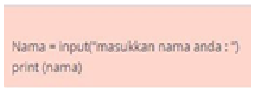
\includegraphics[width=4cm]{figures/1184026/perbedaan1.png}
			\centering
			\caption{input pada python 2}
			\end{figure}
		Pada Python 3, Sintaks yang digunakan untuk mencetak inputan yang digunakan yaitu : 
		\hfill \break
			\begin{figure}[H]
			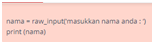
\includegraphics[width=4cm]{figures/1184026/perbedaan2.png}
			\centering
			\caption{input pada python 3}
			\end{figure}
		\item Sintaks yang digunakan dan hasil ketika melakukan operator pembagian\\
\end{itemize}
	\item Implementasi Python dan Penggunaan di Perusahaan Kelas Dunia\\
	Dalam penggunaannya, Python dinyatakan sebagai bahasa pemrograman  yang menggabungkan kemampuan atau kapabilitas dan sintaksis kode yang sangat jelas sehingga mudah dipahami. Selain itu, python juga dilengkapi dengan fungsionalitas pemrograman standar yang besar serta komprehensif. Oleh karenanya, python banyak digunakan oleh perusahaan-perusahaan besar skala nasional maupun internasional.Bukan hanya itu saja python memiliki konsep desain yang sederhana dan bagus sehingga dapat meningkatkan produktivitas programmer serta python juga dapat dijalankan di semua sistem operasi \\
	Berikut ini merupakan beberapa dari banyaknya perusahaan yang menggunakan Python dalam pengembangan usaha mereka, di antaranya yaitu :
	\begin{enumerate}
		\item Instagram
		\item Google
		\item Facebook
	\end{enumerate}
\section{Instalasi}
\begin{itemize}
	\item Instalasi Python\\
	Berikut merupakan urutan yang dilakukan saat melakukan instalasi python, di antaranya yaitu :\\
	\begin{enumerate}
		\item Klik icon Anaconda kemudian klik install atau setup. Setelah itu klik next.
		\begin{figure}[H]
			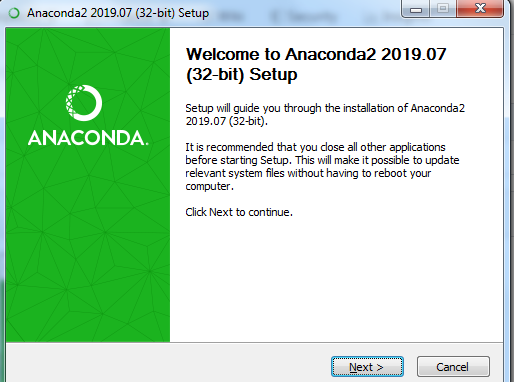
\includegraphics[width=4cm]{figures/1184026/anaconda/anaconda1.png}
			\centering
			\caption{setup anaconda}
			\end{figure}
		\item Setelah itu, klik I agree pada licence agreement.\\
			\begin{figure}[H]
			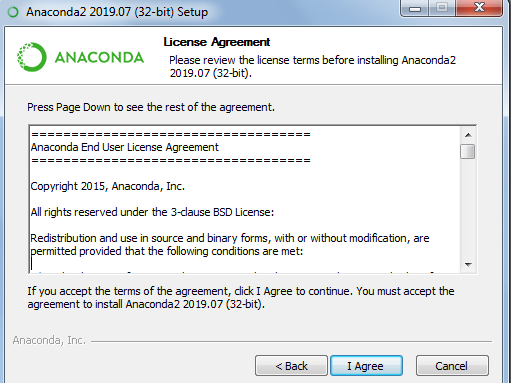
\includegraphics[width=4cm]{figures/1184026/anaconda/anaconda2.png}
			\centering
			\caption{licence agreement}
			\end{figure}
		\item Pilih All User pada installation type, hal ini memungkinkan agar anaconda dapat digunakan oleh semua user pada PC.\\
			\begin{figure}[H]
			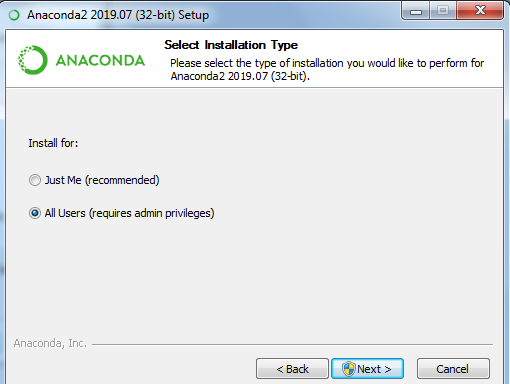
\includegraphics[width=4cm]{figures/1184026/anaconda/anaconda3.png}
			\centering
			\caption{installation type}
			\end{figure}
		\item Pilih lokasi penyimpanan aplikasi Anaconda yang akan diinstal, kemudian klik next.\\
			\begin{figure}[H]
			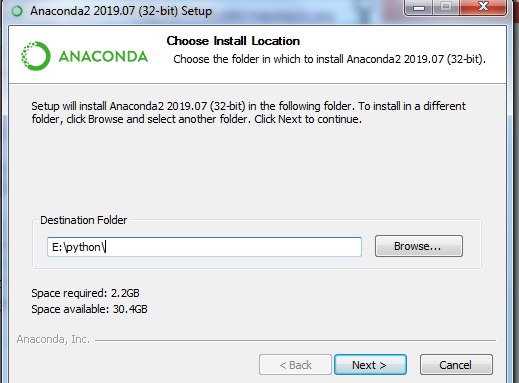
\includegraphics[width=4cm]{figures/1184026/anaconda/anaconda4.png}
			\centering
			\caption{lokasi penyimpanan anaconda}
			\end{figure}
		\item Centang bagian ADD Environtment to the Path walau terdapat notif tidak direkomendasikan, hal ini memungkinkan untuk menambahkan environtment anaconda ke dalam path yang ada dalam PC anda. Setelah itu klik next.
			\begin{figure}[H]
			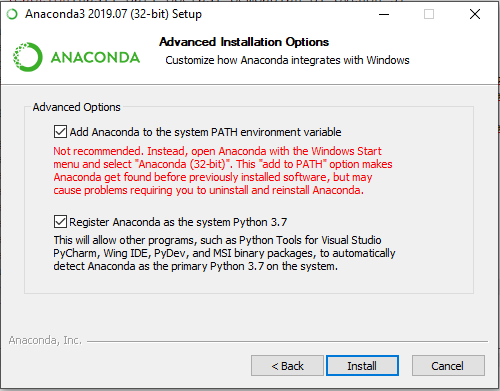
\includegraphics[width=4cm]{figures/1184026/anaconda/anaconda5.png}
			\centering
			\caption{menambahkan path environtment}
			\end{figure}
		\item Tunggu sampai instalasi selesai.
			\begin{figure}[H]
			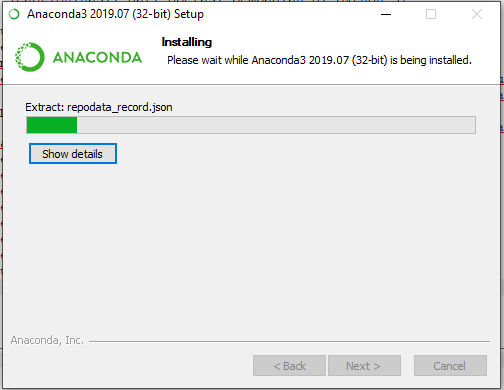
\includegraphics[width=4cm]{figures/1184026/anaconda/anaconda6.png}
			\centering
			\caption{proses instalasi}
			\end{figure}
		\item Setelah Instalasi selesai, maka klik next sampai proses terakhir dan klik finish di akhir proses instalasi seperti pada gambar berikut ini.\\
			\begin{figure}[H]
			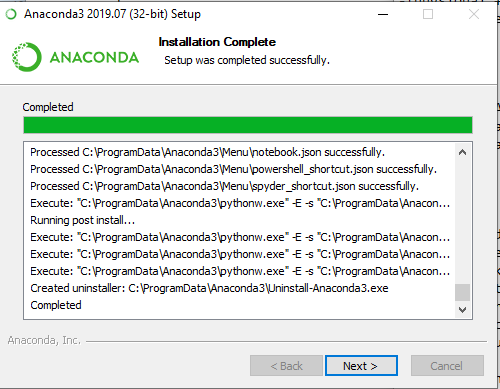
\includegraphics[width=4cm]{figures/1184026/anaconda/anaconda7.png}
			\centering
			\caption{instalasi selesai}
			\end{figure}
			\begin{figure}[H]
			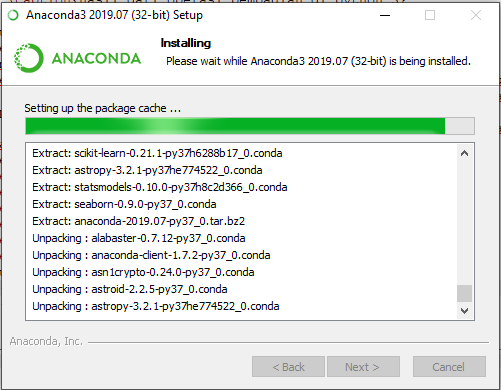
\includegraphics[width=4cm]{figures/1184026/anaconda/anaconda8.png}
			\centering
			\caption{instalasi selesai 2}
			\end{figure}
			\begin{figure}[H]
			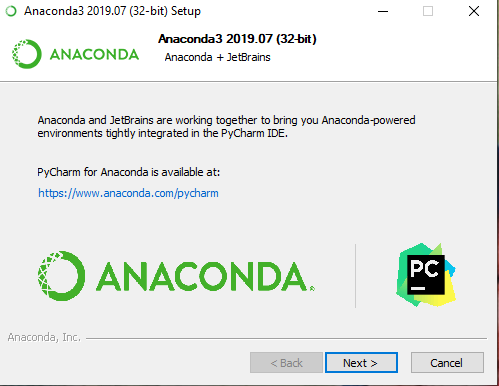
\includegraphics[width=4cm]{figures/1184026/anaconda/anaconda9.png}
			\centering
			\caption{instalasi selesai 3}
			\end{figure}
	\end{enumerate}
	\item Instalasi PIP
		PIP pada dasarnya telah terinstal di dalam Environtment secara otomatis ketika kita sudah melakukan instalasi Python maupun melalui Navigator Anaconda. Langkah awal yang dilakukan untuk menginstalasi PIP yaitu :
		\begin{enumerate}
			\item Download dan update versi pip terbarunya dengan mendownload package dari cmd. Hal ini bisa dilakukan dengan beberapa cara, di antaranya :
			\begin{enumerate}
				\item Ketikkan "curl https://bootstrap.pypa.io/get-pip.py -o get-pip.py". Hasil yang akan didapatkan dapat dilihat seperti gambar berikut ini :
				\begin{figure}[H]
				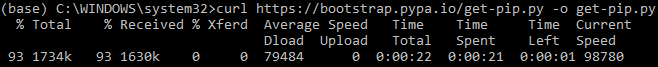
\includegraphics[width=8cm]{figures/1184026/pip/downloadpip.png}
				\centering
				\caption{mendownload pakage pip yang ada}
				\end{figure}
				\item Menggunakan ketikan "pip install -U pip"
				\begin{figure}[H]
				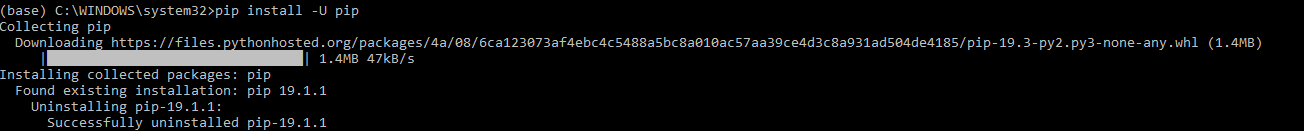
\includegraphics[width=8cm]{figures/1184026/pip/upgrdpip.png}
				\centering
				\caption{mendownload dan mengupgrade versi pip}
				\end{figure}
				\item Dengan mengetikkan "python -m pip install --upgrade pip"
				\begin{figure}[H]
				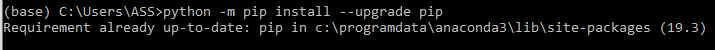
\includegraphics[width=8cm]{figures/1184026/pip/upgrd3.png}
				\centering
				\caption{mendownload dan mengupgrade versi pip 2}
				\end{figure}
			\end{enumerate}
		\end{enumerate}
	\item Setting Environtment
		\begin{enumerate}
			\item Buka My Computer lalu klik kanan dan pilih properties
				\begin{figure}[H]
				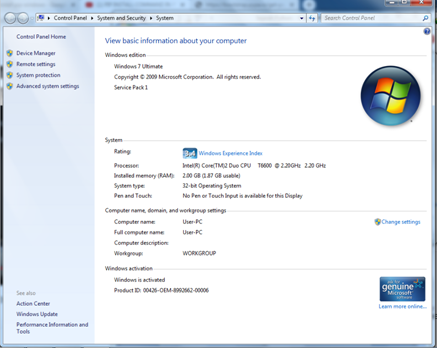
\includegraphics[width=8cm]{figures/1184026/environtment/1.png}
				\centering
				\caption{update anaconda}
				\end{figure}
			\item Pilih advanced system setting
				\begin{figure}[H]
				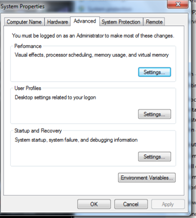
\includegraphics[width=8cm]{figures/1184026/environtment/2.png}
				\centering
				\caption{update anaconda}
				\end{figure}
			\item Kemudian pilih environtment variable
				\begin{figure}[H]
				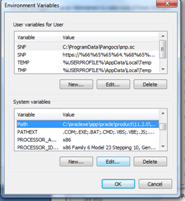
\includegraphics[width=8cm]{figures/1184026/environtment/3.png}
				\centering
				\caption{update anaconda}
				\end{figure}
			\item Pilih Path lalu klik edit
				\begin{figure}[H]
				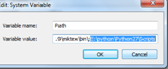
\includegraphics[width=8cm]{figures/1184026/environtment/4.png}
				\centering
				\caption{advance system settings}
				\end{figure}
			\item Ketikan " destinasi folder dimana anaconda di install
				\begin{figure}[H]
				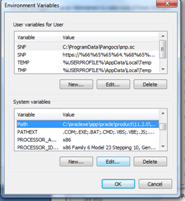
\includegraphics[width=8cm]{figures/1184026/environtment/3.png}
				\centering
				\caption{edit environtment variable}
				\end{figure}
		\end{enumerate}
	\item Mencoba Entrepeter/CLI melalui terminal atau windows
		\begin{enumerate}
			\item Buka cmd kemudian ketikkan python
				\begin{figure}[H]
				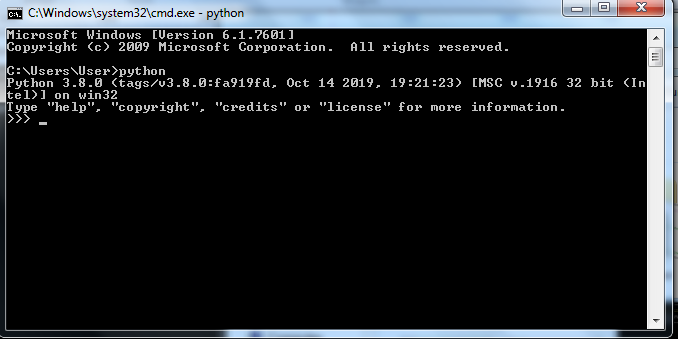
\includegraphics[width=8cm]{figures/1184026/interpreter/1.png}
				\centering
				\caption{tampilan awal cmd setelah diketik "python"}
				\end{figure}
		
			\item ketikkan beberapa sintaks untuk mencoba enterpreter. Disini saya menggunakan sintaks untuk mencetak atau print
				\begin{figure}[H]
				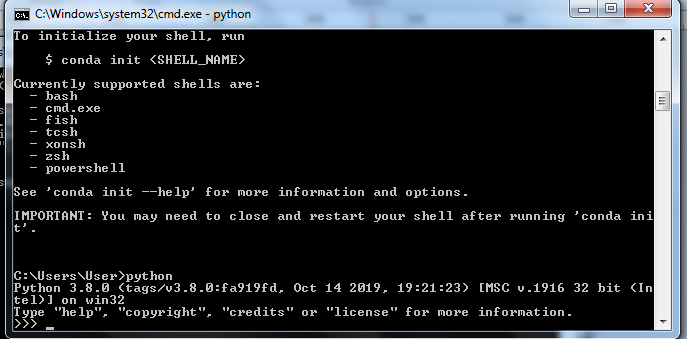
\includegraphics[width=8cm]{figures/1184026/interpreter/4.png}
				\centering
				\caption{hasil mencoba enterpreter di cmd}
				\end{figure}
		\end{enumerate}
	\item Menjalankan dan mengupdate anaconda dan spyder
		Di dalam anaconda ada spyder yang merupakan satu kesatuan karena di dalam navigator anaconda terdapat IDE Spyder. Oleh karenanya dengan mengupdate anacondanya, maka  spyder juga otomatis langsung terupdate. Berikut ini merupakan tata cara untuk mengupdate anaconda, di antaranya adalah :
		\begin{enumerate}
			\item buka cmd atau dapat juga melalui Anaconda Prompt
			\item untuk memulai menggunakan cmd, ketikkan python terlebih dahulu
			\item Setelah itu ketikkan exit() untuk keluar dari conda environtment
			\item Ketikkan conda activate untuk mengaktifkan conda environtment
			\item Untuk memulai dengan Anaconda prompt anda bisa langsung ke tahap ini, yakni ketikkan "conda install -c anaconda python" seperti gambar berikut ini
				\begin{figure}[H]
				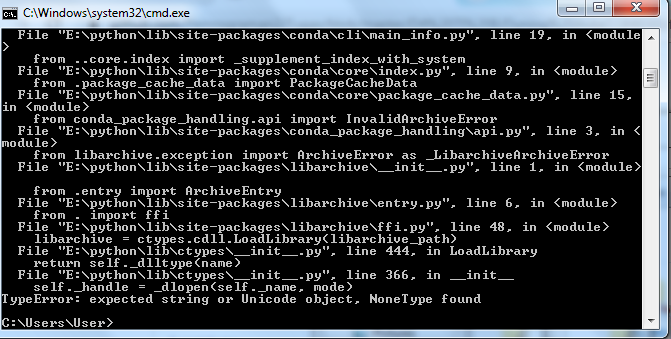
\includegraphics[width=8cm]{figures/1184026/interpreter/6.png}
				\centering
				\caption{install update anaconda}
				\end{figure}
				Setelah proses seperti gambar di atas berjalan, lalu ketikkan "Y" untuk melanjutkan proses. dan sepertinya terjadi eror di laptop saya karena banyak file dll yang belum ada.
		\end{enumerate}
	\item Menjalankan script "Hello World" di Spyder
	 Berikut ini merupakan cara untuk menjalankan script "Hello World", di antaranya yaitu :
	 \begin{enumerate}
	 	\item Buka spyder melalui navigator anaconda yang telah diinstall sebelumnya,biasanya langsung ada di menu start.
	 		
	 	\item Tuliskan script yang akan dibuat
	 		\begin{figure}[H]
			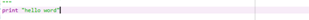
\includegraphics[width=8cm]{figures/1184026/hello.png}
			\centering
			\caption{script hello world}
			\end{figure}
	 	\item ini hasil setelah di running "Hello World"
	 		\begin{figure}[H]
			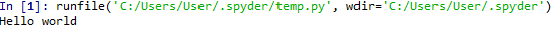
\includegraphics[width=8cm]{figures/1184026/hasil.png}
			\centering
			\caption{tampilan hasil}
			\end{figure}
	 \end{enumerate}
	\item Mengkode dan menjalankan script otomatis untuk login aplikasi akademik dengan library selenium dan inputan user menggunakan mozilla firefox
		Untuk menjalankan script login secara otomatis menggunakan  library selenium diperlukan tahapan sebagai berikut :
		\begin{enumerate}
		\item Buka command prompt kemudian ketikkan "pip install selenium" untuk instalasi paket library selenium ke pc kita
			\begin{figure}[H]
			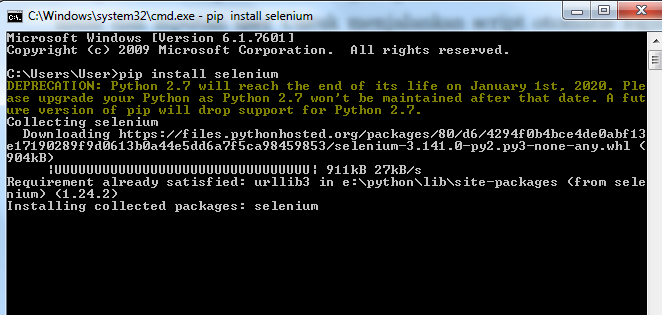
\includegraphics[width=8cm]{figures/1184026/selenium.png}
			\centering
			\caption{install selenium}
			\end{figure}
		\item Download geckodriver.exe sesuai versi yang sesuai spesifikasi pc anda
		\item Masukan geckodriver.exe tersebut ke dalam folder system32 yang ada di dalam local disk c 
		\item Buka IDE Spyder untuk menuliskan script login otomatis
		\item Ketik script perintah selenium yang akan dieksekusi. Berikut script yang dituliskan :
			\begin{figure}[H]
			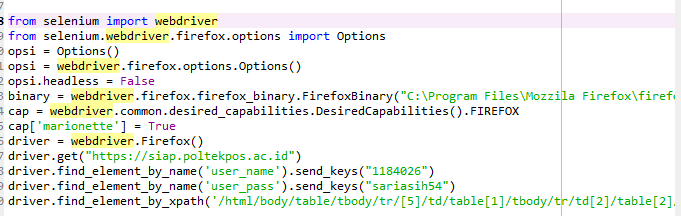
\includegraphics[width=8cm]{figures/1184026/eror/20.png}
			\centering
			\caption{kode script login secara otomatis}
			\end{figure}
		\item Setelah di run maka firefox akan otomatis masuk ke halaman sistem akademik siap dengan menginputkan username dan email yang sesuai inputan dalam script selenium tadi.
			\begin{figure}[H]
			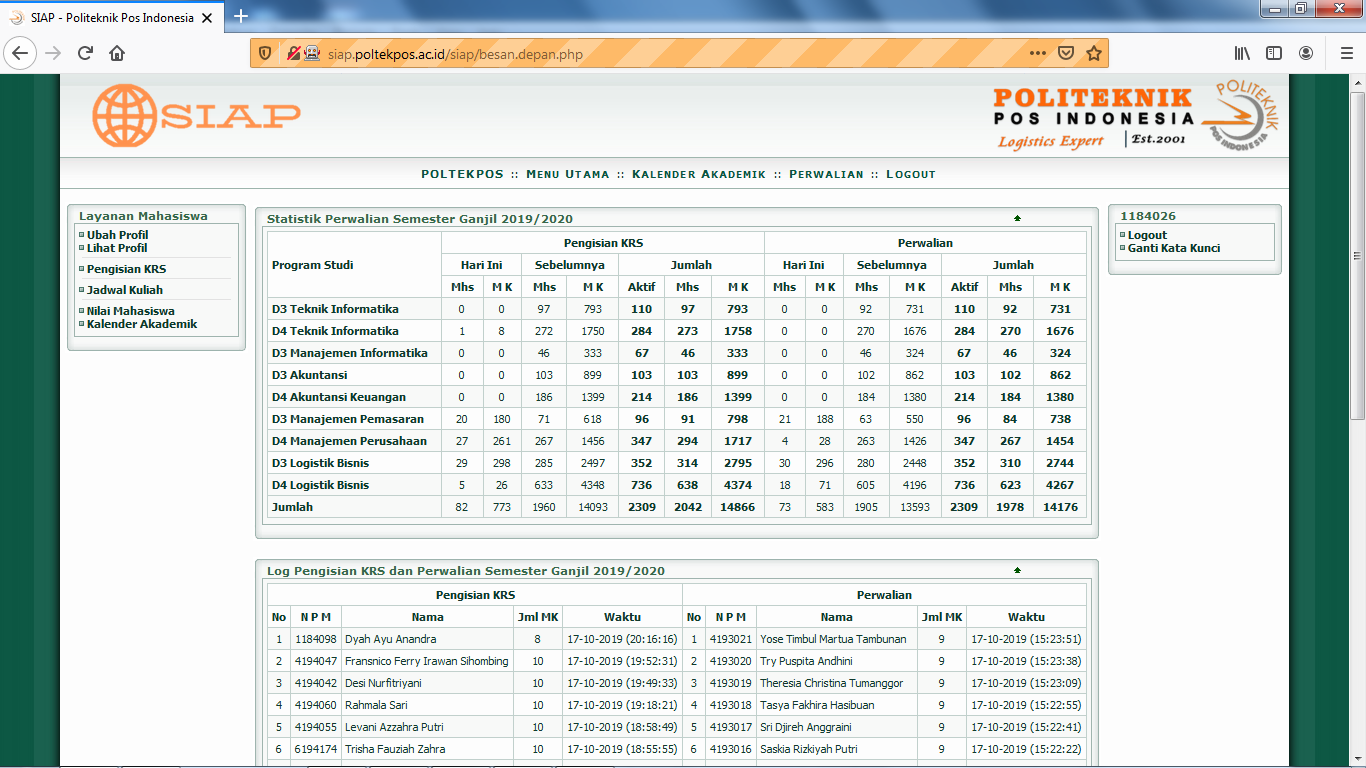
\includegraphics[width=8cm]{figures/1184026/login.png}
			\centering
			\caption{login otomatis ke sistem akademik siap}
			\end{figure}
		\end{enumerate}
		\item Mencoba menggunakan Variable Explorer di Spyder
		\begin{enumerate}
		\item Tulis kode script pada spyder yang mengandung variabel
			\begin{figure}[H]
			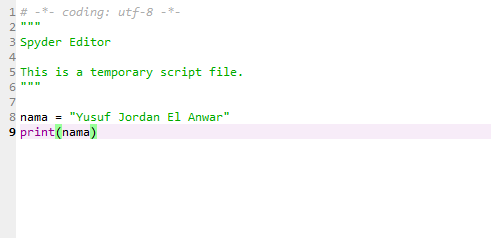
\includegraphics[width=8cm]{figures/1184026/variabel/1.png}
			\centering
			\caption{penulisan variabel}
			\end{figure}
		\item Run kode tersebut, maka nama, tipe, dan nilai akan ditampilkan  di menu variabel explorer yang ada di sisi kanan bagian atas.
			\begin{figure}[H]
			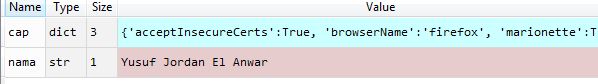
\includegraphics[width=8cm]{figures/1184026/variabel/2.png}
			\centering
			\caption{tampilan variabel explorer}
			\end{figure}
		\item Pada ipython console akan tertera hasil dari script yang diketik sebelumnya
		\item Untuk mengedit variabel yang telah dibuat sebelumnya, klik kanan pada variabel explorer. Maka akan dimunculkan tampilan seperti berikut ini
			\begin{figure}[H]
			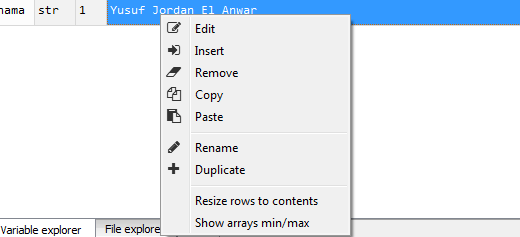
\includegraphics[width=8cm]{figures/1184026/variabel/3.png}
			\centering
			\caption{edit variabel}
			\end{figure}
		\end{enumerate}
\end{itemize}
\section{Identasi}
\begin{itemize}
	\item Penjelasan Identasi
		Indentasi berasal dari kosa kata dalam bahasa Inggris Indentation yang bermakna memindahkan atau mendorong ke dalam. Hal itu berati bahwa menjorokkan script kode ke dalam merupakan indentasi. Indentasi di dalam bahasa python digunakan sebagai penanda blok program, sedangkan pada umumnya indentasi digunakan untuk mempermudah dalam membaca script kode yang telah dibuat. Oleh karenanya, indentasi di dalam script python sangatlah penting dan bisa menyebabkan terjadinya error jika kita tidak mengetahui cara untuk menggunakannya.
	\item Jenis-jenis error identasi yang didapat
			Jenis error indentasi yang biasa terjadi ada 12 keadaan dalam bahasa pemrograman yang berbeda-beda. Pada bahasa pemrograman python, jenis error indentasi yang terjadi adalah ketika kita salah atau tidak memberi identasi atau menjorok pada script. Hal itu dikarenakan pada bahasa pemrograman python, indentasi adalah penanda blok program.
	\item Cara membaca error yang ada pada identasi
	\begin{enumerate}
	\item Lihat pada jendela script pada bagian samping. Jika terdapat tanda warning atau tanda silang, maka hal itu menandakan bahwa terdapat error pada script yang anda buat
			\begin{figure}[H]
			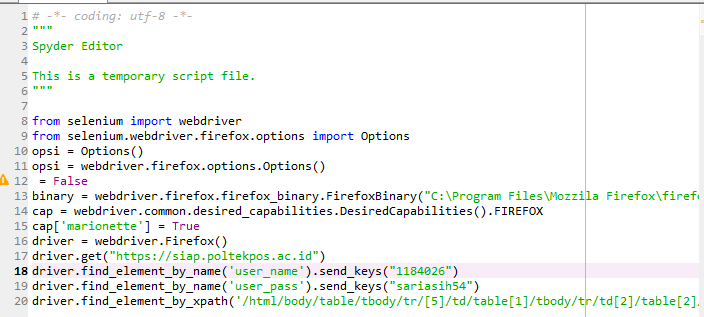
\includegraphics[width=8cm]{figures/1184026/eror/1.png}
			\centering
			\caption{error indentasi}
			\end{figure}
	\item Selain itu, lihat pada jendela iPython Console. Jika terdapat error maka saat script dijalankan maka akan menampilkan warning untuk menampilkan bagian mana yang salah seperti berikut
			\begin{figure}[H]
			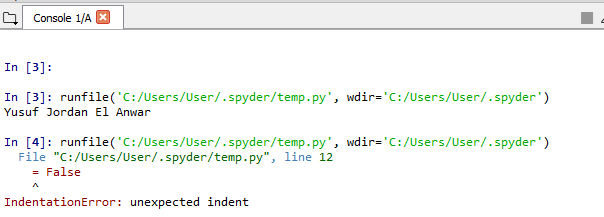
\includegraphics[width=8cm]{figures/1184026/eror/2.png}
			\centering
			\caption{error indentasi pada console}
			\end{figure}
	\end{enumerate}
	\item Cara menangani error yang terjadi
	\begin{enumerate}
		\item Cek ke baris yang dituju, yakni baris yang terdapat tanda warning seperti gambar dibawah ini
			\begin{figure}[H]
			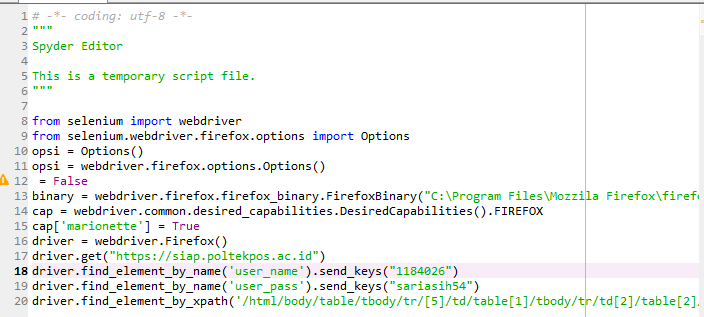
\includegraphics[width=8cm]{figures/1184026/eror/1.png}
			\centering
			\caption{error indentasi pada console}
			\end{figure}
		\item Perhatikan Warning kesalahan yang muncul pada jendela iPython Console terhadap baris karena warning kuning dan merah memilki arti yang berbeda tersebut
			\begin{figure}[H]
			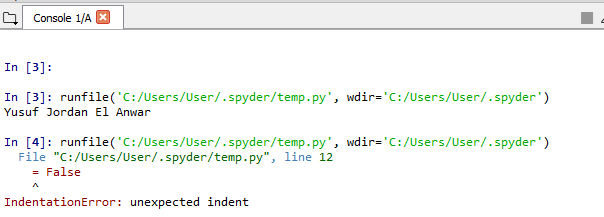
\includegraphics[width=8cm]{figures/1184026/eror/2.png}
			\centering
			\caption{error indentasi pada console}
			\end{figure}
		\item jika perbaiakan kesalahan sudah benar maka  tanda warning pada line tersebut menghilang
			\begin{figure}[H]
			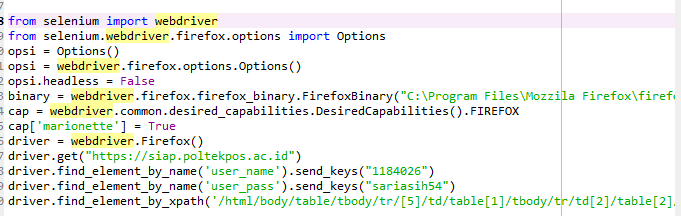
\includegraphics[width=8cm]{figures/1184026/eror/20.png}
			\centering
			\caption{error yang telah diperbaiki}
			\end{figure}
		\item Run kembali script yang dituju
	\end{enumerate}
\end{itemize}
\end{enumerate}